\documentclass{article}

\usepackage[a4paper]{geometry}
\usepackage{graphicx}
\usepackage{hyperref}
\usepackage[utf8]{inputenc}
\usepackage{subcaption}

\graphicspath{{./images/}}

\title{\textbf{WizardGame}}
\author{
    Dumitru Mițca\\
    Faculty of Automatic Control and Computer Engineering, Iași\\
    dumitru.mitca@student.tuiasi.ro}
\date{2022-2023}

\begin{document}
    \maketitle

    \begin{figure}[h]
        \begin{subfigure}{0.5\linewidth}
            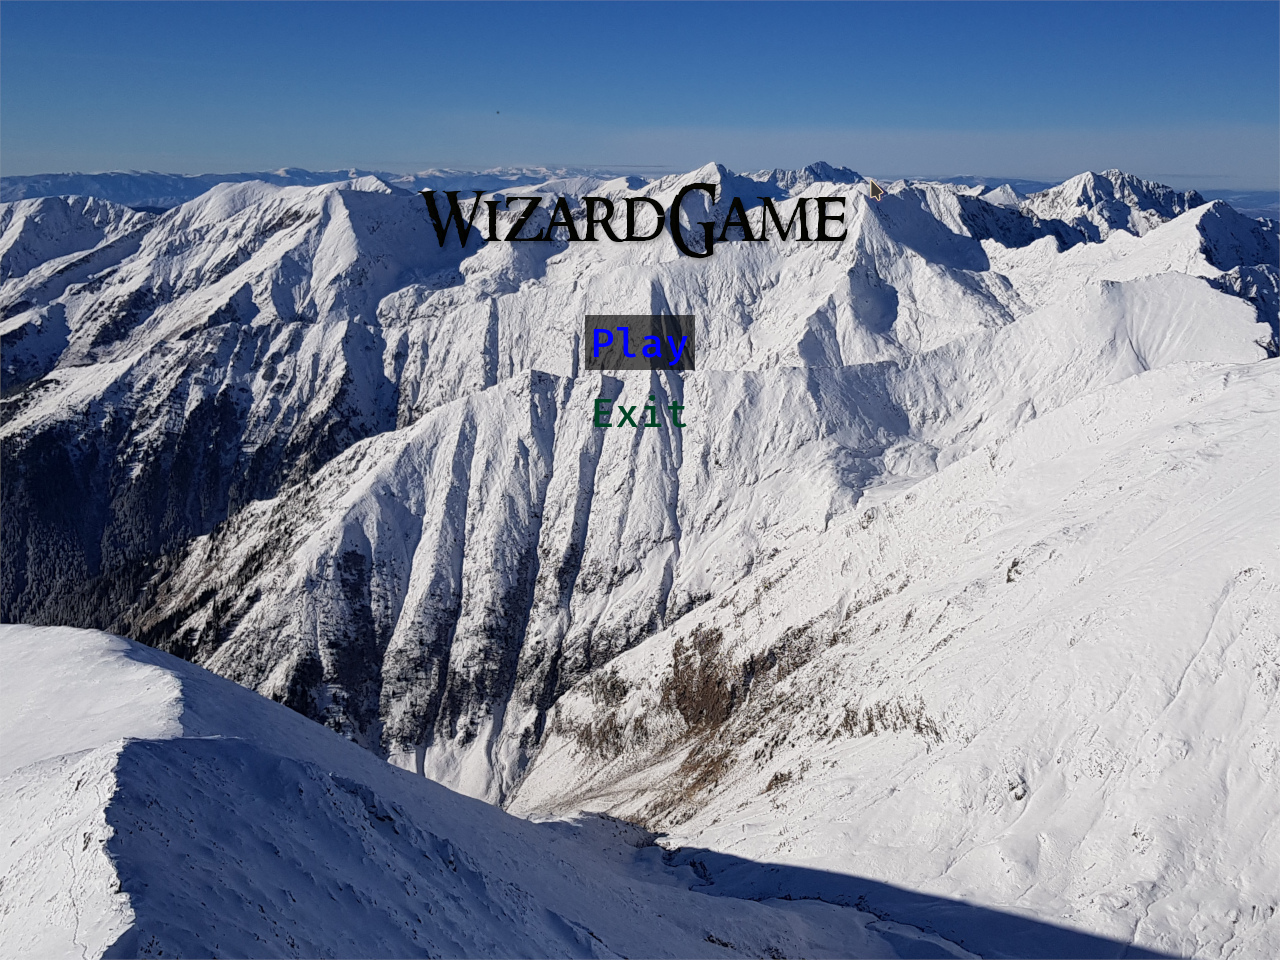
\includegraphics[width=\linewidth]{main-menu}
            \caption{The main menu}
        \end{subfigure}
        \begin{subfigure}{0.5\linewidth}
            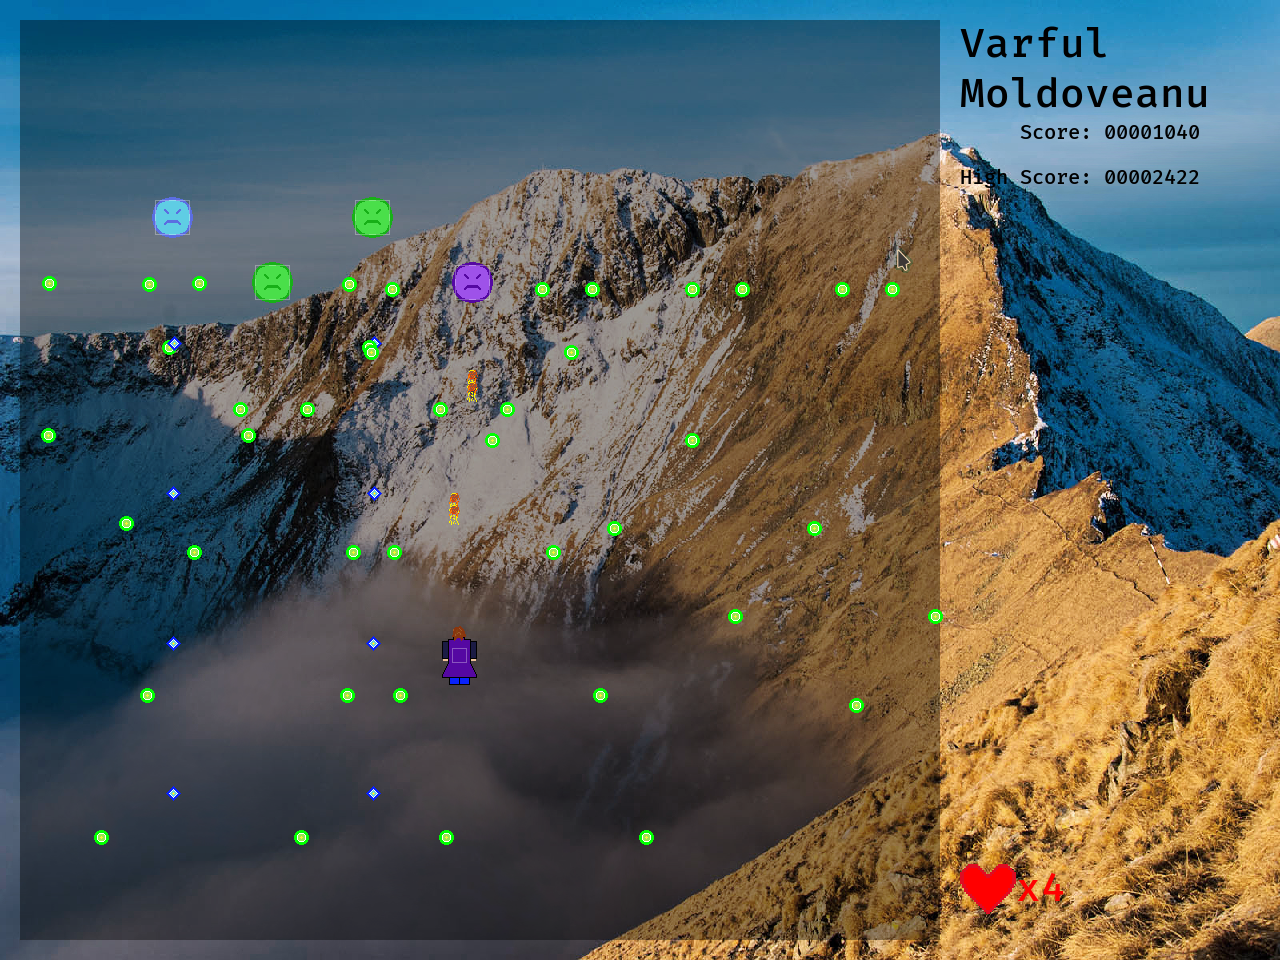
\includegraphics[width=\linewidth]{level}
            \caption{Fighting Adrian}
        \end{subfigure}
    \end{figure}

    The source code of the game can be found at \url{https://github.com/RealKC/WizardGame}.

    \section{Gameplay}

    The game consists of a single player campaign composed of a tutorial and 3 levels of increasing
    difficulty in which the player must kill various enemies in order to win the game.

    The gameplay consists of the player shooting projectiles at (mostly stationary) enemies and having
    to dodge the projectiles shot by the enemies. Enemies can shoot projectiles in various patterns
    (one at a time, three at once, semicircle, and a special star shaped attack for the boss), however
    the player is limited to a simple one at a time attack pattern, but can do so at an increased rate
    compared to enemies. Though simple, this gameplay can have a high skill ceiling, as demonstrated
    by other games in this genre.

    \section{Plot}

    In the year 1964, Adrian, the Shaman of Neamț, has announced to the magic world that he
    shall destory the Carpathian Mountains and used a powerful spell to steal the magic books of
    every other wizard in Romania. Only Mircea, the Wizard of Brăila, the best fire magician in the
    country, is able to save the Carpathians now. Using the spell he can cast without seeing the
    runes --- fireball --- he shall stop Adrian from his evil plan.

    \section{Characters}
    \begin{itemize}
        \item \textbf{Mircea}, \emph{The Wizard of Brăila} --- the protagonist and player character
        of the game, he wishes to stop Adrian from accomplishing his destructive goal.
        \item \textbf{Adrian}, \emph{The Shaman of Neamț} --- the antagonist, he wishes to
        destroy the Carpathians to avenge the singer Michael Jackson, who had been killed at a concert
        held in the Carphatian Mountains.
        \item \textbf{Matei}, \emph{The Sensei} --- Mircea's mentor, he tragically dies in the tutorial.
        \item \textbf{Mihai} --- Mircea's best friend and a fellow fire magician. He has lost his hand
        in the war of 1959 and is thus unable to help Mircea battle Adrian.
    \end{itemize}

    \section{Mechanics}
    \begin{itemize}
        \item \emph{Lives} --- the player has a limited number of lives (5), which are decreased when
        the player is hit by a projectile; once it reaches zero, the player loses all progress in the
        current level and must try again.
        \item \emph{Score} --- the game tracks your score as you kill enemies, but halves it for every
        recorded death.
        \item \emph{Waves} --- each level is split in multiple waves, a wave contains enemies that must
        be defeated in order to progress, and you must beat all waves of a level to progress further in
        the game.
    \end{itemize}
\end{document}
